\documentclass{oxmathproblems}
\usepackage{algorithm}
\usepackage{algpseudocode}


\course{Algorithm Design and Analysis}
\sheettitle{Assignment 5 \\ Wu Jiabao, 523030910241} %can leave out if no title per sheet

\begin{document}
\begin{questions}
\miquestion
Denote the primal $A$ as $A_0$ and it is modified to $A_1$.\\
If $A_1$ is invertible, we can transform $A_1$ into $E$ by elementary transformation. Thus there exist $n$ entries with value $1$ such that no two entries are in the same row and no two entires are in the same column.\\
If these $n$ entries exist, modify other entries to $0$. Then the column vectors of $A_1$ are linear independent, making $A_1$ invertible.

\begin{algorithm}[h]
\caption{Maximum Matching}
\textbf{Input:} A $n\times n$ matrix $A$ whose entries are either $0$ or $1$\\
\textbf{Output:} Whether $A$ is invertible after modification
\begin{algorithmic}[1]
    \State $L\gets$ the column vectors of $A$\;
    \State $R\gets$ the row vectors of $A$\;
    \State draw an edge between row vertex $i$ and column vertex $j$ \textbf{if} $a_{ij}=1$\;
    \State employ \textbf{Edmonds-Karp Algorithm} on $L$ and $R$ to find the maximum matching\;
    \State \textbf{return} whether the maximum matching size is $n$
\end{algorithmic}
\end{algorithm}
\textbf{Proof of Correctness:} In the algorithm above we find the maximum matching between the row vectors and column vectors. 
Since in the matching one row can only match at most one column and vice versa, if the size of maximum matching is $n$, we can find $n$ unique pairs that none of their rows are the same and their columns neither.
From the theorem above we know that it is possible to make $A$ invertible after modification.

\textbf{Time Complexity:} $O(n^5)$ derived from Edmonds-Karp Algorithm $O(|E|^2|V|)$.

\miquestion
\begin{parts}
\part
\begin{algorithm}[h]
    \caption{Maximum Matching}
    \textbf{Input:} a ground set $U$ and a collection of subsets $\mathcal{A}$\\
    \textbf{Output:} whether $\mathcal{A}$ has a system of distinct representatives
    \begin{algorithmic}[1]
        \State $L\gets$ elements of $\mathcal{A}$\;
        \State $R\gets$ elements of the ground set $U$\;
        \State draw an edge between subset $A_i$ and a ground element $u_j$ if $u_j\in A_i$\;
        \State employ \textbf{Edmonds-Karp Algorithm} on $L$ and $R$ to find the maximum matching\;
        \State \textbf{return} whether the maximum matching size is $k$
    \end{algorithmic}
    \end{algorithm}
\textbf{Proof of Correctness:} If the size of matching is $k$, $k$ distinct elements from $U$ match to $k$ subsets in $\mathcal{A}$. 
So we can select these elements to construct a system of distinct representatives.\\
If the size of matching is not $k$, there exists at least one subset such that we cannot find a distinct element. Thus $\mathcal{A}$ does not have a system of distinct representatives.

\textbf{Time Complexity:} $O(n^3k^2)$ derived from Edmonds-Karp Algorithm $O(|E|^2|V|)$.

\part
Construct a graph as the figure shows.
\begin{figure}[h]
    \centering
    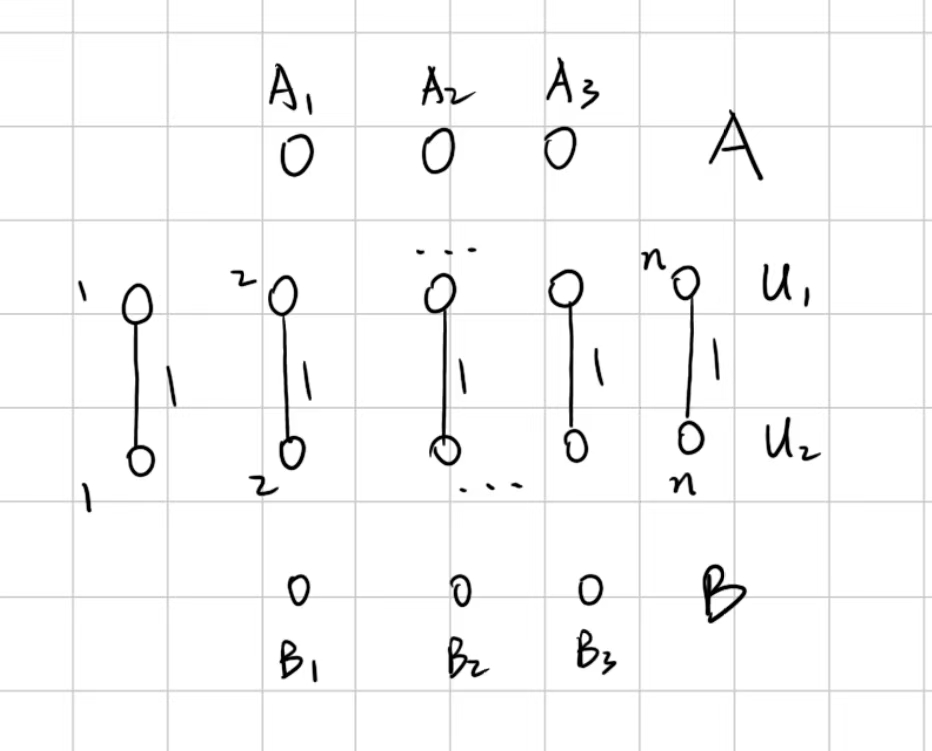
\includegraphics[scale=0.25]{2(b)graph.jpg}
    \caption{finding common system of distinct representatives}
\end{figure}
\begin{algorithm}[h]
    \caption{Maximum Matching}
    \textbf{Input:} the graph shown above\\
    \textbf{Output:} whether $\mathcal{A}$ and $\mathcal{B}$ have a common system of distinct representatives
    \begin{algorithmic}[1]
        \State draw an edge between $A_i$ and $u_j\in U_1$ if $u_j\in A_i$\;
        \State draw an edge between $B_i$ and $u_j\in U_2$ if $u_j\in B_i$\;
        \State employ \textbf{Edmonds-Karp Algorithm} on the graph to find the maximum matching\;
        \State \textbf{return} whether the maximum matching size is $k$
    \end{algorithmic}
\end{algorithm}

\textbf{Proof of Correctness:} $U_1$ and $U_2$ ensure that for each element in $U$, it will be selected at most once. 
Otherwise the flow between $U_i\in U_1$ and $u_i\in U_2$ is larger than $1$.\\
Assume the maximum matching size is less than $k$ and the common system of distinct representatives exists. 
Then we can find $T$ with $k$ distinct elements that is the system of distinct representatives of both $\mathcal{A}$ and $\mathcal{B}$. 
However, we cannot find such $T$ since the size is less than $k$. Contradiction!\\
If the maximum matching size is $k$, we can find $k$ distinct elements in both $\mathcal{A}\hbox{ and }\mathcal{B}$. Thus the common system of distinct representatives exists.

\textbf{Time Complexity:} $O(k^2n^3)$ since Edmonds-Karp Algorithm costs $O(|E|^2|V|)$.
\end{parts}

\miquestion
\begin{parts}
\part
Assume $|A|=n>m=|B|$. Since every vertex has the same degree(denoted as $d$) and it is a bipartate graph, we know $nd=|E|=md$. Contradiction!\\
It is the same with $|A|<|B|$, so $|A|=|B|$.
\part
\textbf{Base case:} Obviously the theorem holds for $d=1$.\\
\textbf{Inductive hypothesis:} Assume the theorem holds for $d=k-1$.\\
For $d=k-1$, add $n$ edges to make each vertex's degree be $k$. Since $G$ has already contained a matching of size $n$, adding edges does not affect the size of this matching. 
thus we can always find a matching of size $n$ when $d=k$.\\
\textbf{Conclusion:} Therefore, $G$ must contain a matching of size $n$.
\end{parts}

\miquestion
\begin{parts}
\part
Relace $x_e\geq0$ to $x_e\in\{0,1\}$. Let $e=(u,v)$ be the edge between $u$ and $v$, $x_e$ be whether $u$ matches with $v$ or not. 
Then the problem can be explained as:
\begin{align*}
    \text{maximize }& \sum_{e\in E}x_e\\ &\text{(maximize the size of matching)}\\
    \text{subject to }&\sum_{e:e=(u,v)}x_e\leq 1\tag{$\forall v\in V$}\\  &\text{($u$ can only match with one vertex at most)}\\
    &x_e\in\{0,1\}\tag{$\forall e\in E$}\\ &\text{($x_e$ determines whether $u$ matches with $v$ or not)}
\end{align*}
It is equal to the difinition of the maximum matching problem. Thus the linear program describes \emph{the fractional version} of the maximum matching problem.

\part
\begin{align*}
    \text{minimize }& \sum_{u\in V}x_u\\
    \text{subject to }& x_u+x_v\geq 1 \tag{$\forall(u,v)\in E$}\\
    &x_u\geq0 \tag{$\forall u\in V$}
\end{align*}
Repalce $x_u\geq0$ to $x_u\in\{0,1\}$. Consider $x_u$ as whether $u$ is selected or not. Then the target function is minimizing the size of vertex cover. 
The first subjective function indicates that for each edge in $E$, at least one of its endpoints is a vertex cover. 
The last subjective function determines that for each vertex $u$, $x_u$ denotes whether it is selected as vertex cover or not. 
Thus this dual program describes the fractional version of the minimum vertex cover problem.

\part
\textbf{Base step:} each cell of $A$ belongs to $\{0,1\}$.\\
\textbf{Inductive step:} Assume every $k\times k$ submatrix of $A$ has determinant belongs to $\{0,1,-1\}$. Consider any $(k+1)\times(k+1)$ submatrix $A'$.
\begin{itemize}
    \item \textbf{Case 1:} If a column of $A'$ is all-zero, then $det(A')=0$.\;
    \item \textbf{Case 2:} If a column of $A'$ contains only one non-zero entry, then $det(A')$ equals to $\pm1$ times the determinant of a $k\times k$ submatrix. $det(A')\in\{0,1,-1\}$ by induction hypothesis.\;
    \item \textbf{Case 3:} If every column of $A'$ has two non-zero entries(both of them are $1$), we can divide the matrix into two parts $X$ and $Y$. Adding all the row vectors in $X$ and $Y$, we get two same vectors with all their components are $1$. Thus $det(A)=0$.
\end{itemize}
Therefore, $A$ is totally unimodular.

\part
Since in the maximum matching problem and minimum vertex cover problem, $x_e$ and $x_u$ are integral, and $A$ is totally unimodular, we know that both the primal and dual problem have integral optimal solutions. 
From the strong dual theorem we can conclude that the size of the maximum matching equals to the size of minimum vertex cover in a bipartate graph.

\part
Triangle. Its size of maximum matching is $1$ while minimum vertex cover is $2$.
\end{parts}

\miquestion
\begin{parts}
\part
Denote $d_f(u)$ as the minimum distance from $t$ to $u$ in the flow $f$.\\
Consider a augmented path $p=(s,\cdots,u,v,\cdots,t)$ in $G'_{L}$. Obviously $d_{f'}(s)\geq d_f(s)$. The equality holds while $d_f(u)=d_f(v)+1$.\\
Assume $d_{f'}(s)=d_f(s)$. From a augmented path from $s$ to $t$ in $G_L'$, we can find an edge $(u,v)$ such that is not in $G_L$. Otherwise from $d_f(s)=d_{f'}(s)$ we know that the blocking flow on $G_L$ has not been found yet. 
Since $(u,v)\notin G_L$, we have:\\
\textbf{case 1:} $(u,v)\in E_f$ but $d_f(u)<d_f(v)+1$. From the definition of level graph we know $(u,v)\notin E_L$.\\
\textbf{case 2:} $(u,v)\notin E_f$, thus it is a reverse edge, $d_f(u)=d_f(v)-1$.\\
From the two cases we know $d_f(u)\neq d_f(v)+1$, then $d_{f'}(s)>d_f(s)$. So the distance from $s$ to $t$ is strictly monotonically increasing.
\part
\begin{algorithm}[h]
    \caption{Compute a blocking flow on a level graph}
    \textbf{Input:} a level graph $G_L$\\
    \textbf{Output:} a blocking flow on $G_L$
    \begin{algorithmic}[1]
        \State emplpoy DFS on $s$ to find a path to $t$\;
        \State \textbf{during} DFS:\;
        \State \hspace{0.5cm} skip iterating an edge $(u,v)$ if $v$'s incident edges are blocked\;
        \State find a path from $s$ to $t$ and select the minimum capacity as the flow on this path\;
        \State combine these flows together to get a blocking flow\;
    \end{algorithmic}
\end{algorithm}
Each time we find a augmented flow, there is at least one edge in $E_L$ is blocked. Collect these edges in the set $E_1$. Since $G_L$ is a level graph, the reverse edge of $E_1$ will not be visited by other augmented flows in this iteration. Thus $E_1\subset E_L$.\\
Consider such condition that we fail to find a augmented flow due to the level of the graph is at most $|V|$. Collect the last edge of these path in the set $E_2$. Since it is not a augmented flow, $E_1\cup E_2\subset E_L$.\\
For each DFS to find a augmented flow, it costs $O(|V|)$ due to skiping some edges. Thus finding a blocking flow on a level graph costs $O(|V||E_L|)=O(|V||E|)$. 
\part
Since after each iteration, the distance from $s$ to $t$ in $G^f$ is increased by at least $1$, the iteration must be less than $|V|$ because the level of the level graph is less than $|V|$. 
Each iteration costs $O(|V|\cdot|E|)$ and iterate $O(|V|)$ times. The total time complexity of Dinic's Algorithm is $O(|V|^2\cdot|E|)$.
\end{parts}
\miquestion
It takes me about 8 hours to finish the homework. Difficulty is 4. Collaborators: Li Haochen, Wang Kun.
\end{questions}

\end{document}
